\begin{frame}{Consistency-based methods \cite{saeed2009overview}}

    \begin{itemize}    
        \item Based on: “prevention is the best medicine”
        \item Combines iterative and progressive approaches with probabilistic models:
        \begin{enumerate}
        \renewcommand{\baselinestretch}{2}
        \item Uses \textbf{\underline{Hidden Markov Models}} to calculate matrices for matching residues in pairwise alignments. 
        \item Uses information about multiple sequence alignment as it is being generated to guide the pairwise alignments.
        \item Multiple alignment via tree-based \textbf{\underline{progressive alignment}}
        \item Errors at early stages in the alignment are alleviated by \textbf{\underline{post-processing steps}} such as iterative refinement. See \cite{wallace2005multiple}.
        \end{enumerate}

    \end{itemize}
    
\end{frame}

\begin{frame}{Consistency-based methods}

    \begin{block}{Imaging this biological scenario \cite{pevsner2015bioinformatics}}
    \centering
            \large Sequence x $\rightarrow$ $ x_{i}$ \\
            \large Sequence y $\rightarrow$ $ y_{i}$ \\
            \large Sequence z $\rightarrow$ $ z_{k}$ \\
    \end{block}
    \centering
    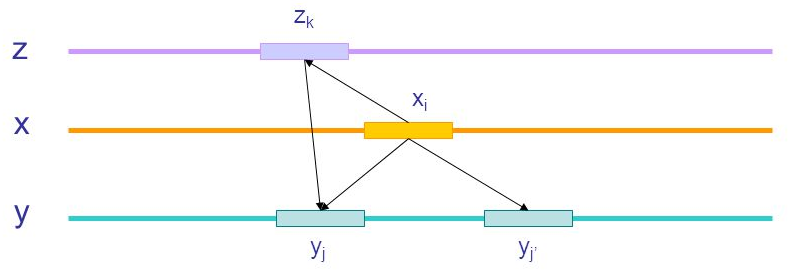
\includegraphics[width=0.65\linewidth]{img/xyz.PNG}
    \begin{itemize}
        \item If $ x_{i}$ aligns with $ z_{k}$ and $ z_{k}$ aligns with $ y_{i}$, then $x_{i}$ should align with $ y_{i}$
    \end{itemize}
    \begin{itemize}
            \item Consistency-based techniques \textbf{score pairwise alignments} in the context of \textbf{information about multiple sequences}
    \end{itemize}
\end{frame}